
\section{LV and HV Tape, Supply and Cable Losses}

\subsection{Low voltage}
\label{low_voltage}

\begin{figure}[ht!]
\begin{center}
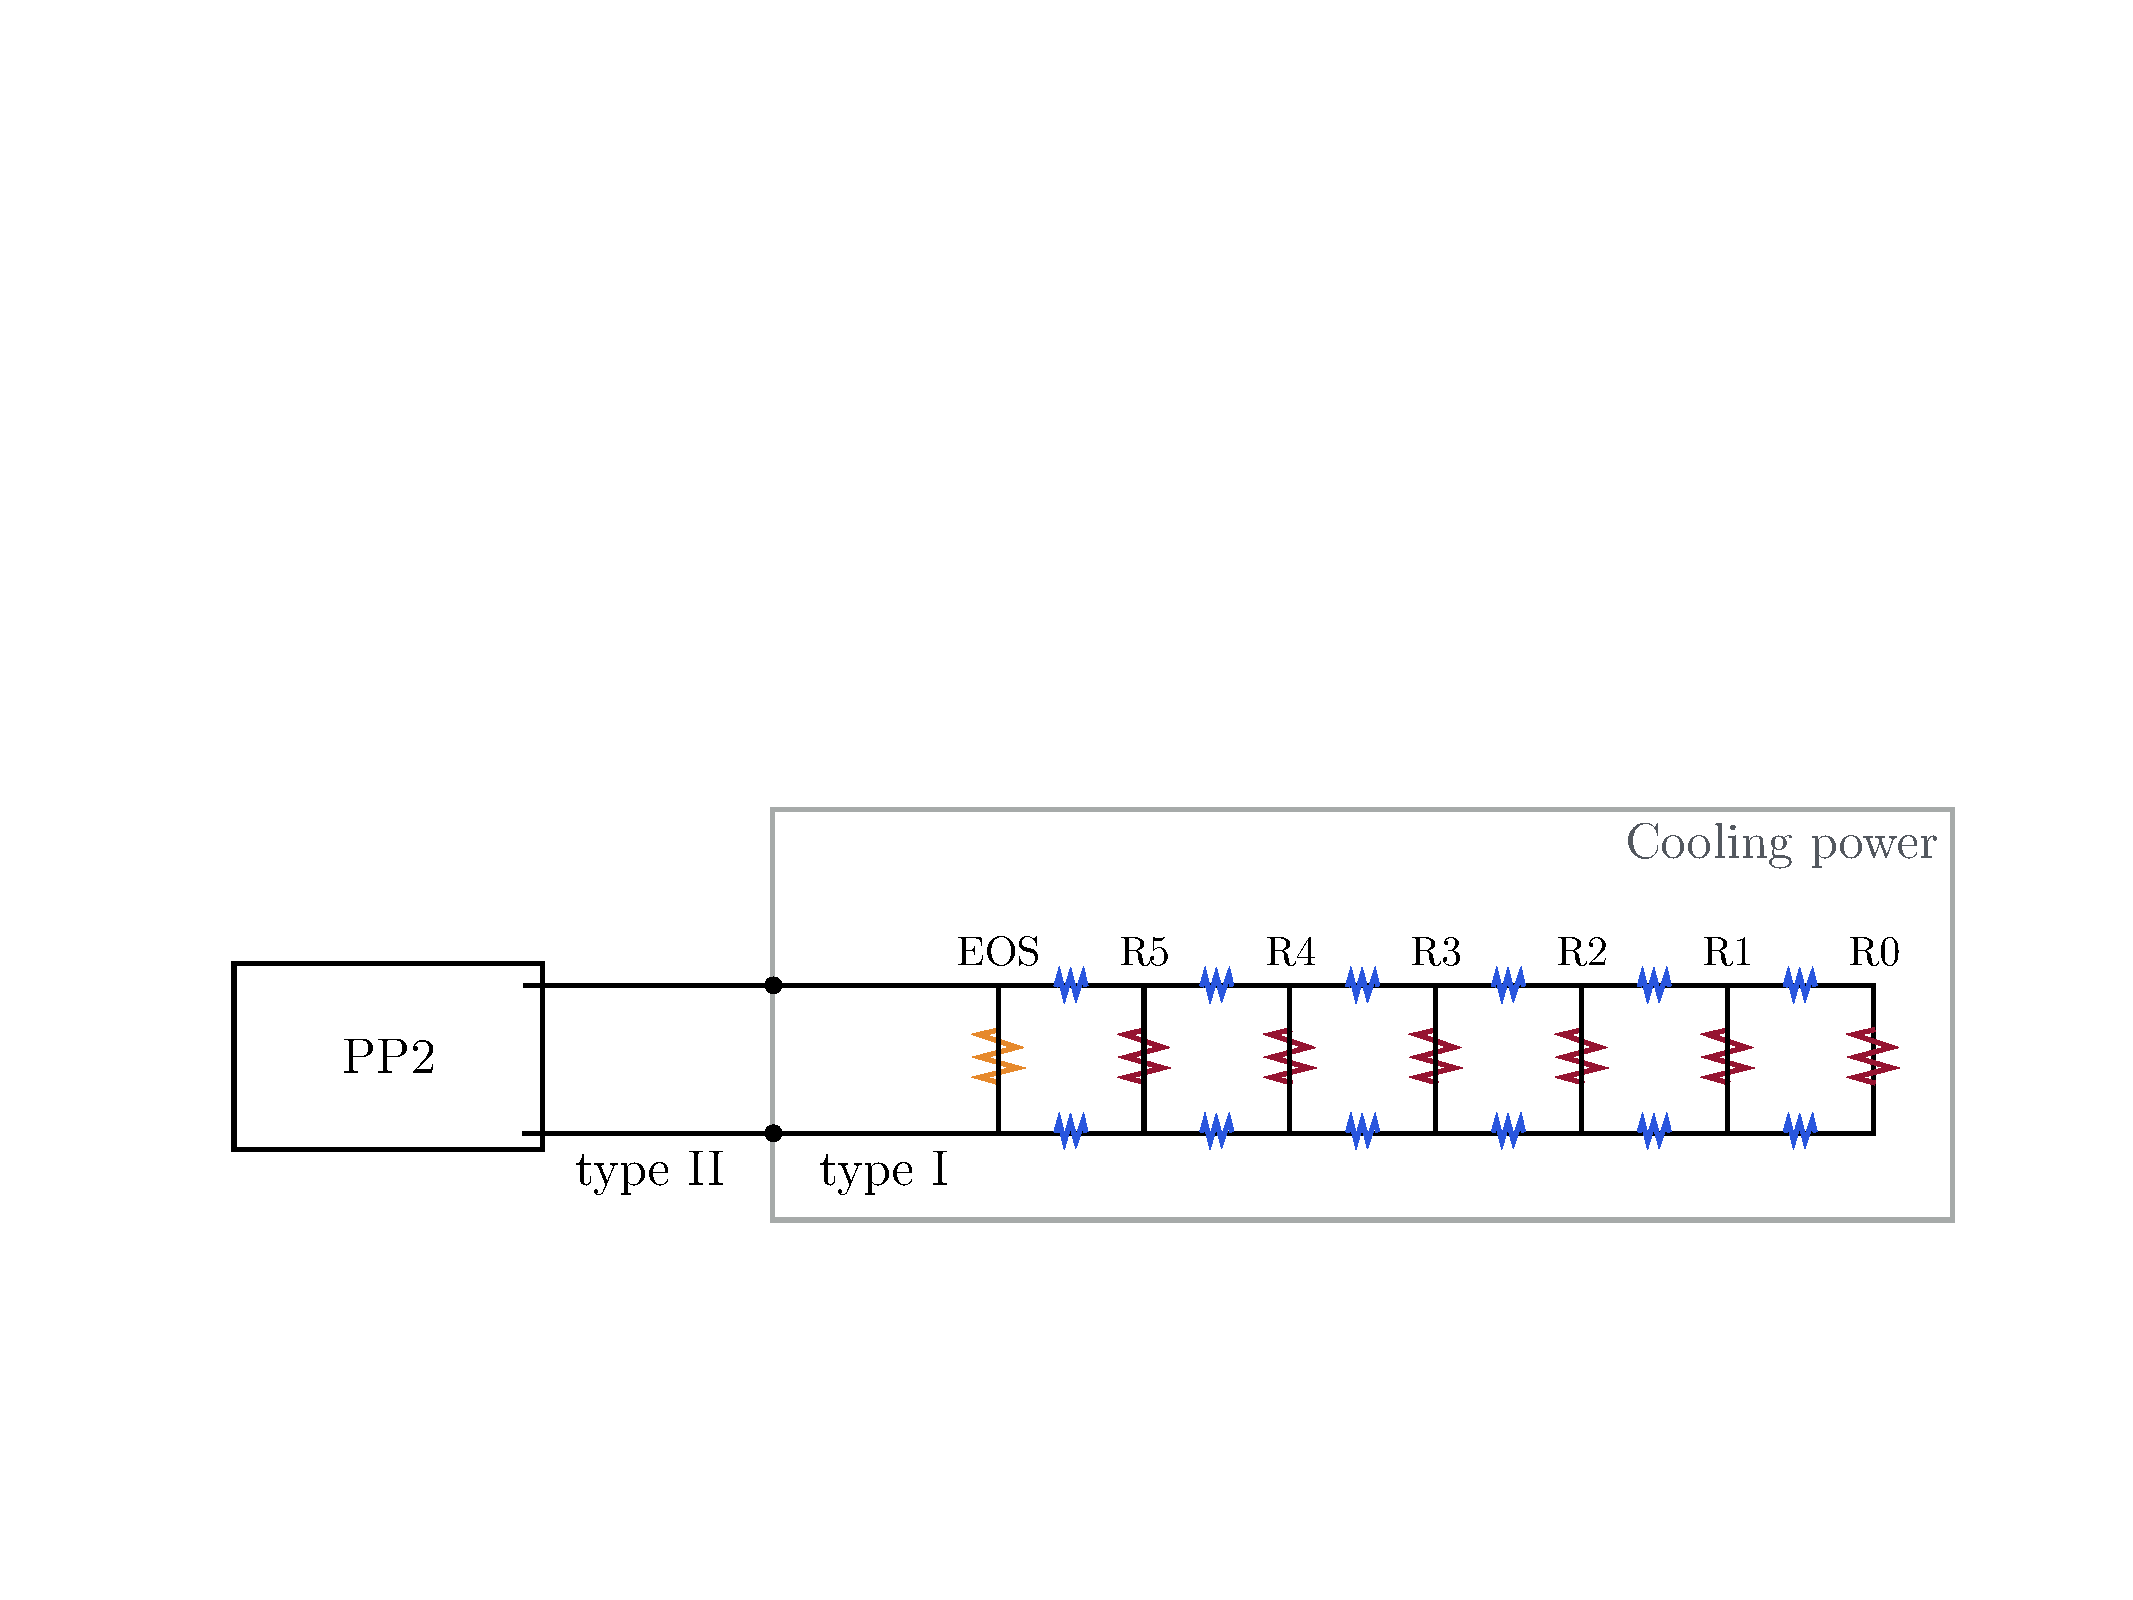
\includegraphics[width=0.74\linewidth]{figures/LV_cartoon.pdf}
\end{center}
\caption{Simplified depcition of the petal LV circuit. The EOS effective resistance is in orange;
the voltage drop from BPOL12V and linPOL12V is in red; the tape resistance is blue.
The type-I cables are counted in the cooling power.}
\label{lv_circuit}
\end{figure}

Figure~\ref{lv_circuit} depicts a simplified version of the LV circuit.

%% The low-voltage is modeled as losing 1V over the length of the petal, with 11V at the EOS and
%% dropping to 10V in R1\footnote{Estimates provided by Pepe Bernabeu.} at beginning-of-life.
%% To ensure consistency between
%% the tape resistance and the voltage drop in the front-end components in each module, (and because I
%% don't have good numbers for endcap tape resistances), tape resistance values are chosen to cause a
%% 1/6~V drop between modules.


The low-voltage will be sensed at the EOS at 11 V, and expected to drop up to 1 V through the length of
the tape, depending on the tape resistance. Estimates of the tape resistance are under investigation;
for now a worst-case tape resistance of 20 m$\Omega$ is used in the endcap.

To ensure consistency between
the tape resistance and the voltage drop in the front-end components in each module,
the voltage drop in the R0 front-end is strategically chosen such that the $\Delta V$
of the R0 front-end plus the total tape $\Delta V$ equals 11 V at the EOS.
The procedure is as follows:
to correctly model the tape current and LV voltage in each module, the model performs its predictions
of each module starting from R0, followed by R1, R2, ... R5. The voltage drop across the front-end
components in R0 is set at 10.79~V. The current in the R0 tape is:
%
\[
I^{R0}_\text{tape} = \frac{P^{R0}_{LV}}{V^{R0}_{LV}}.
\]
When calculating the next-highest module (e.g. R1), the FE voltage is set to the voltage drop of the
previous FE, plus the additional voltage drop due to the tape in the previous module:
\[
V^{Rn}_{LV} = V^{R(n-1)}_{LV} + I^{R(n-1)}_\text{tape} R^{R(n-1)}_\text{tape}.
\]
Likewise, the tape current in module $Rn$ is equal to the current from the module's FE plus the
accumulated current from the previous modules:
\[
I^{Rn}_\text{tape} = \frac{P^{Rn}_{LV}}{V^{Rn}_{LV}} + I^{R(n-1)}_\text{tape}.
\]
With $\Delta V$ at R0 set at 10.79~V, the voltage at the EOS is 11~V in beginning-of-life conditions
(without safety factors).
Note that this calculation occurs at each time step in the model, so power increases due to the TID
bump affect both the FE voltages and the tape current.
(The effect of the bump is less than 0.1~V at the TID bump maximum.)

Table~\ref{voltage_drops} specifies the voltage input at each module given the
chosen tape resistance value of 20~m$\Omega$.

\begin{table}[ht]
\begin{center}
\adjustbox{max width=\textwidth}{ %% just before tabular
\begin{tabular}{|l|l|r|r|r|r|r|r|l|} \hline % data_below
Quantity & Description           &     R0 &     R1 &     R2 &     R3 &     R4 &     R5 & Unit   \\ \hline
\multirow{2}{*}{$V_{in}$} & Input voltage to the BPOL12V &  \multirow{2}{*}{10.79} &  \multirow{2}{*}{10.80} &  \multirow{2}{*}{10.82}
&  \multirow{2}{*}{10.85} &  \multirow{2}{*}{10.89} &  \multirow{2}{*}{10.94} & \multirow{2}{*}{V}      \\
 & and linPOL12V on each module & & & & & & & \\ \hline
$R_\text{tape}$           & Tape resistance in each module &  \multicolumn{6}{c|}{20} & m$\Omega$ \\
\hline\end{tabular}
} %% resize box after tabular
\end{center}
\caption{Voltage inputs for each endcap module. The EOS is assumed to have an 11V input voltage.}
\label{voltage_drops}
\end{table}

\subsection{Low voltage cables}

The low-voltage power calculations follow Georg's treatment, with the exception of the
calculations of module voltages described above.
Several quantities are quoted in the main summary tables:
following Figure~\ref{lv_circuit}, the
quantity ``LV round-trip $\Delta V$ from PP2'' consists of voltage drops from type I and II cables
only, and ``Max LV $V_\text{out}$ at PP2'' represents the voltage drop of the tape plus FE
($\Delta V_{R0} + \Delta V_\text{tape}$), plus the voltage drop of the type I and II cables.

\subsection{High voltage}

% https://edms.cern.ch/ui/file/1889475/10/Bus_Tapes_specs_v10_300118.pdf
%% There will be 4 separate HV lines for barrel and petals. For the petals, the
%% separate HV lines will serve modules: R5, R4, R3 and R2, and R1 and R0. For the
%% barrels, the HV lines will serve modules: 0 to 3, 4 to 7, 8 to 10 and 11 to 13, where
%% module 0 is defined to be the module closest to the centre of the detector and module 13
%% is adjacent to the EoS.

\begin{figure}[ht!]
\begin{center}
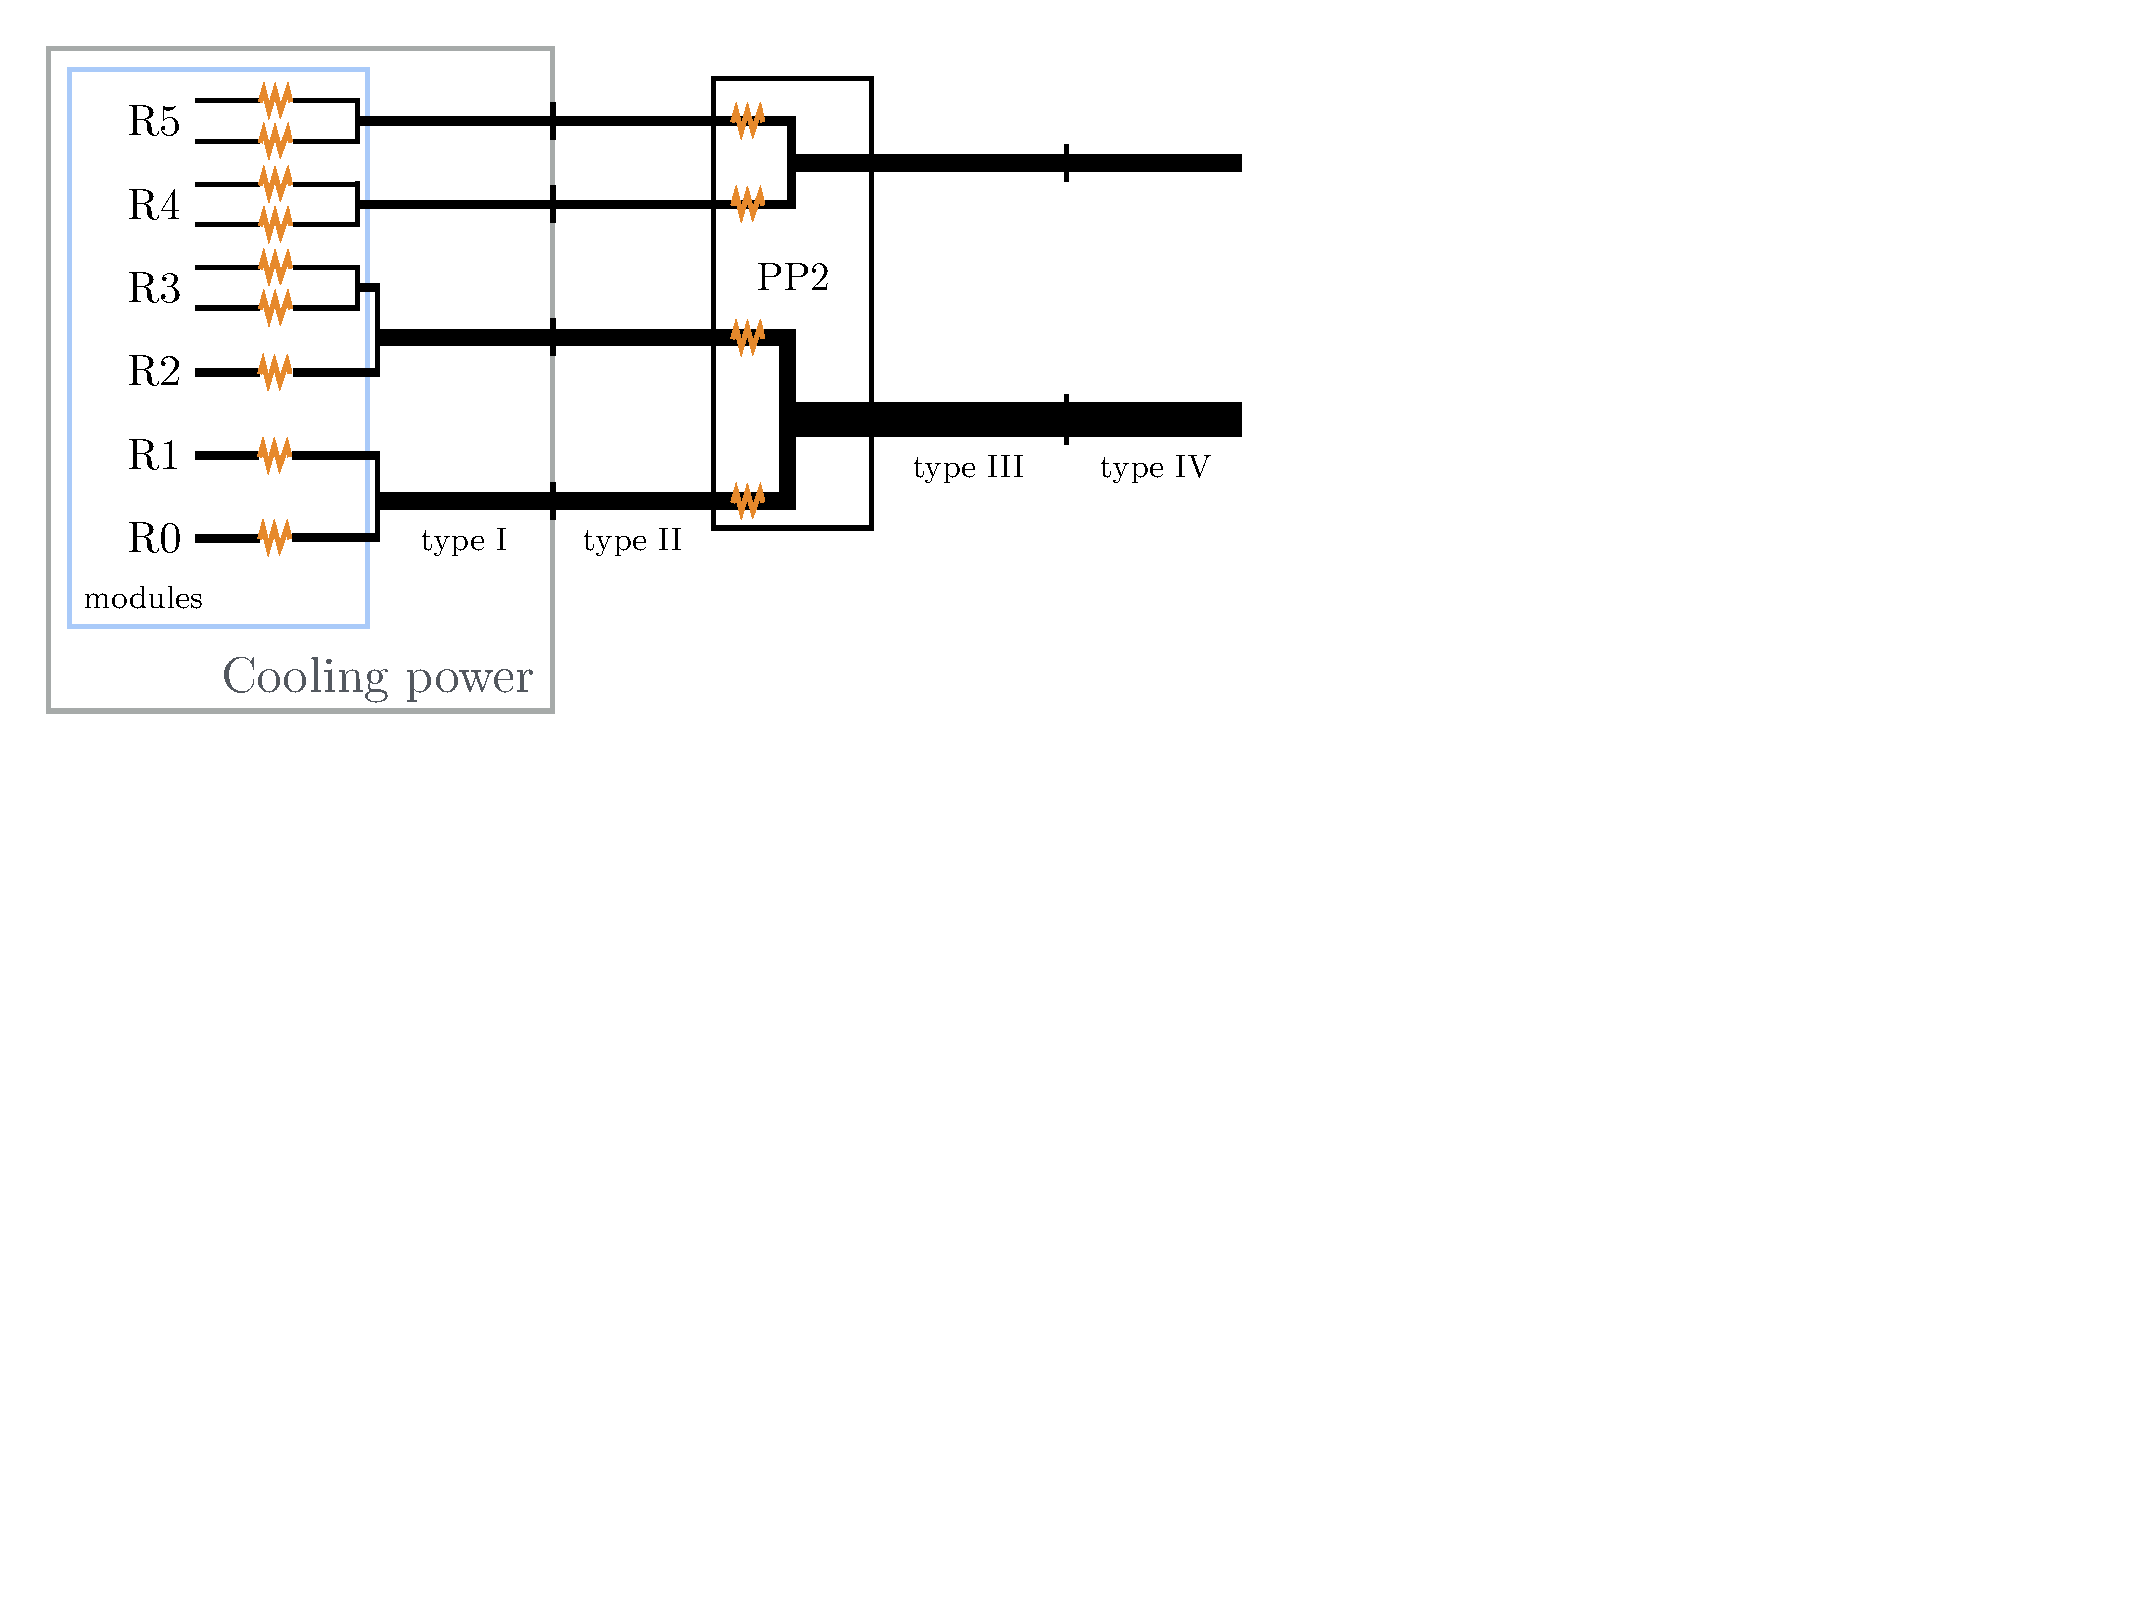
\includegraphics[width=0.60\linewidth]{figures/HV_cartoon.pdf}
\end{center}
\caption{Simplified depcition of the petal HV circuit, showing the HV cable multiplexing scheme. HV filters are shown
in orange. The type-I cables are counted in the cooling power. The HV return current will use the LV return line.}
\label{hv_circuit}
\end{figure}

Figure~\ref{hv_circuit} depicts a simplified version of the HV circuit. Most of the treatment of the
HV voltage and power calculations use the same strategies and equations described in Georg's text, with
the exceptions described below.
{ \bf Important note: the endcap HV tape resistance is currently set to 0. } The expected impact on petal
and total power results is very small.

\def\rhvmuxI{R^\text{HV,cables}_\text{muxI/II}}
\def\rhvmuxIII{R^\text{HV,cables}_\text{muxIII/IV}}

There are four Type I and II HV lines per petal side, which serve modules in the following multiplexing
scheme: (R0 + R1), (R2 + R3), R4, R5\footnote{ See
https://edms.cern.ch/ui/file/1889475/10/Bus\_Tapes\_specs\_v10\_300118.pdf
}. The HV tape and PP2 HV filters are also assumed to be multiplexed in this way. Thus, we can define
a quantity $\rhvmuxI$ to refer to the sum of these resistances:
%
\def\rtape{R^\text{HV}_\text{tape}}
\def\rtypeI{R^\text{HV}_\text{typeI}}
\def\rtypeII{R^\text{HV}_\text{typeII}}
\def\rtypeIII{R^\text{HV}_\text{typeIII}}
\def\rtypeIV{R^\text{HV}_\text{typeIV}}
\[
\rhvmuxI = \rtape + \rtypeI + \rtypeII + R^\text{HV}_\text{PP2}
\]

The multiplexing of the Type III and IV cables is currently
assumed to be (R0 + R1 + R2 + R3) and (R4 + R5). We can define an effective resistance for these
too:
\[
\rhvmuxIII = \rtypeIII + \rtypeIV
\]

Then the HV voltage drops of the services (including the filters on the module) are then:
\def\dvservices{\Delta V^\text{services}}
\begin{align}
\dvservices_\text{HV,R0} =& I^{R0}_S \cdot R_{HV}           + \left(\sum_{X=0,1} I^\text{RX}_S\right) \cdot \rhvmuxI + \left(\sum^3_{X=0} I^\text{RX}_S\right) \cdot \rhvmuxIII \\
\dvservices_\text{HV,R1} =& I^{R1}_S \cdot R_{HV}           + \left(\sum_{X=0,1} I^\text{RX}_S\right) \cdot \rhvmuxI + \left(\sum^3_{X=0} I^\text{RX}_S\right) \cdot \rhvmuxIII \\
\dvservices_\text{HV,R2} =& I^{R2}_S \cdot R_{HV}           + \left(\sum_{X=2,3} I^\text{RX}_S\right) \cdot \rhvmuxI + \left(\sum^3_{X=0} I^\text{RX}_S\right) \cdot \rhvmuxIII \\
\dvservices_\text{HV,R3} =& I^{R3}_S \cdot \frac{R_{HV}}{2} + \left(\sum_{X=2,3} I^\text{RX}_S\right) \cdot \rhvmuxI + \left(\sum^3_{X=0} I^\text{RX}_S\right) \cdot \rhvmuxIII \\
\dvservices_\text{HV,R4} =&                                I^{R4}_S \cdot \left(\frac{R_{HV}}{2} +\rhvmuxI \right)   + \left(\sum_{X=4,5} I^\text{RX}_S\right) \cdot \rhvmuxIII \\
\dvservices_\text{HV,R5} =&                                I^{R5}_S \cdot \left(\frac{R_{HV}}{2} +\rhvmuxI \right)   + \left(\sum_{X=4,5} I^\text{RX}_S\right) \cdot \rhvmuxIII
\end{align}
%
where the contribution from the on-module HV filter is halved in R3, R4 and R5 because of the
two-filter, split-current scheme in those modules.

The HV power dissipated in the HV services, excluding the on-module HV filters (whose power is counted
as part of the module), is:
\def\phvservices{P^\text{services}_\text{HV}}
\[
\phvservices = \rhvmuxI \cdot \left[ \left(\sum_{X=0,1} I^\text{RX}_S\right)^2
                                    +\left(\sum_{X=2,3} I^\text{RX}_S\right)^2
                                    +\left(I^{R4}_S\right)^2
                                    +\left(I^{R5}_S\right)^2
                                    \right]
               + \rhvmuxIII \cdot \left[ \left(\sum^3_{X=0} I^\text{RX}_S\right)^2
                                        +\left(\sum_{X=4,5} I^\text{RX}_S\right)^2
                                        \right]
\]

Table~\ref{cableHVInputs} describes the cable inputs used for the HV power losses.
Note that the HV return current will use the LV return line, meaning the cable one-way
length is not doubled in the HV case when calculating $\Delta V_\text{HV}$ and $\phvservices$.

\begin{table}[ht]
\begin{center}
\adjustbox{max width=\textwidth}{ %% just before tabular
\begin{tabular}{|l|l|r|l|} \hline % data_below
Configurable Item         & Description                          &      Value & Unit        \\ \hline
HVType1ResistancePerMeter & Type 1 HV cable resistance per meter &      0.213 & $\Omega$/m  \\
HVType2ResistancePerMeter & Type 2 HV cable resistance per meter &      0.213 & $\Omega$/m  \\
HVType3ResistancePerMeter & Type 3 HV cable resistance per meter &      0.139 & $\Omega$/m  \\
HVType4ResistancePerMeter & Type 4 HV cable resistance per meter &    0.14286 & $\Omega$/m  \\
LVType1ResistancePerMeter & Type 1 LV cable resistance per meter &   0.025438 & $\Omega$/m  \\
LVType2ResistancePerMeter & Type 2 LV cable resistance per meter &     0.0148 & $\Omega$/m  \\
LVType3ResistancePerMeter & Type 3 LV cable resistance per meter &     0.0095 & $\Omega$/m  \\
LVType4ResistancePerMeter & Type 4 LV cable resistance per meter &    0.00127 & $\Omega$/m  \\
PP2Efficiency             & PP2 Efficiency                       &       0.85 &             \\
PP2HVFilterResistance     & PP2 Efficiency                       &      100.0 & $\Omega$    \\
PP2InputVoltage           & PP2 input voltage                    &       48.0 & V           \\
PowerSuppliesEfficency    & Power supplies efficiency            &        0.8 &             \\
Type1LengthOneWay         & Type 1 LV/HV cable one-way length    &        2.6 & m           \\
Type2LengthOneWay         & Type 2 LV/HV cable one-way length    &       15.0 & m           \\
Type3LengthOneWay         & Type 3 LV/HV cable one-way length    &       32.0 & m           \\
Type4LengthOneWay         & Type 4 LV/HV cable one-way length    &       70.0 & m           \\
HV tape resistance        & HV tape resistance                   &        0.0 & $\Omega$    \\
\hline\end{tabular}
} %% resize box after tabular
\end{center}
\caption{HV cable inputs for the endcap}
\label{cableHVInputs}
\end{table}
